\documentclass{article}
\usepackage{amsmath, amssymb, graphicx}
\usepackage[margin=1in]{geometry}
\title{CMPS 142: Homework Assignment 3}
\author{Jeffrey Petersen - 1329242\\Ben LASTNAME- ID\\Raymond Colebaugh - 1377877}
\begin{document}
\maketitle
\begin{enumerate}
        \item 
        \item
            In executing grid search with the specified bounds on parameters, we
            determined the following costs and gammas for SMO, where $X$ is the 
            cost and $y$ is $\gamma$:
            $$ \begin{tabular}{c c c c c c | c}
                $c_{ min }$ & $c_{ max }$ & $c_{ step }$ & $\gamma_{ min }$ & $\gamma_{ max }$ & $\gamma_{ step }$ & Accuracy \\ \hline
                   1    &   16    &    1     &       -5     &     2        &        1
            \end{tabular} $$
            Where the expression for $c$ was $i$ and the expression for $\gamma$ was $10^i$.
        \item
            We can demonstrate the construction of a decision tree on a simple
            binary dataset such as:
            $$ \begin{tabular}{c c | c}
                $x_1$ & $x_2$ & $y$ \\ \hline
                0 & 1 & 1 \\
                1 & 1 & 1 \\
                1 & 0 & 0 \\
                0 & 0 & 1 \\
                1 & 0 & 0   % <-
            \end{tabular} $$
            In calculating the decision tree, we first decide the attribute to split
            on for the first node by finding the sum the incorrect predictions. Should we split
            on $x_1$, when $x_1 = 0$ there are no errors, and when $x_1 = 1$ there are
            two errors. Should we split on $x_2$, if $x_2 = 0$ we have one error, and
            if $x_2 = 1$ we have no errors. This makes a split on $x_2$ the better choice.
            Then for the second node, should $x_2 = 0$, we split on the remaining attribute,
            $x_1$. By following decision tree algorithm, we find a representation in the
            following tree:
            $$ 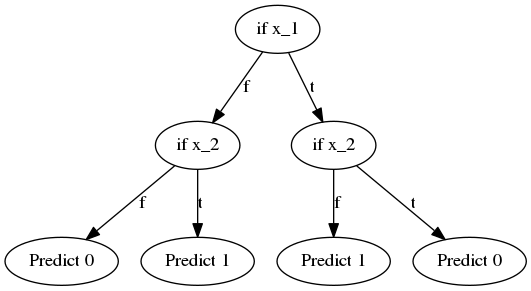
\includegraphics[scale=0.5]{3-1.png} $$
            However, there exists a simpler tree to classify this miniscule dataset,
            should we allow compound conditionals on the nodes:
            $$ 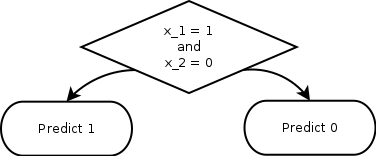
\includegraphics[scale=0.5]{3-2.png} $$
\end{enumerate}
\end{document}
